\documentclass{article}

% Márgenes.
\usepackage{geometry}
\addtolength{\hoffset}{-0.2cm}
\addtolength{\textwidth}{0.4cm}
\addtolength{\voffset}{-0.5cm}
\addtolength{\textheight}{1cm}

% Multicolumnas
\usepackage{multicol}

% Caracteres especiales del español.
\usepackage[utf8]{inputenc}

% Para el lenguaje español.
\usepackage[spanish]{babel}

% Símbolos matemáticos
\usepackage{amssymb}

% Binomio de Newton.
\usepackage{amsmath}

% Imágenes
\usepackage{graphicx}
\graphicspath{ {./img/} }

% SVG
\usepackage{svg}

% Algoritmos
\usepackage[ruled,vlined,linesnumbered]{algorithm2e}

% Para que los figuras se queden en su lugar.
\usepackage{float}

% Macros.
\newcommand{\tbf}[1]{\textbf{#1}}

\newcommand{\tit}[1]{\textit{#1}}

\newcommand{\ttt}[1]{\texttt{#1}}

\newcommand{\np}{\mathcal{NP}}

% Título y autor del reporte.
\title{Uso de la Heurística de Aceptación por Umbrales para Resolver
       el Problema de la Cubierta de Vertices (Vertex Cover)}
\author{Carrasco-Ruiz Mauricio  \\
	maucarrui@ciencias.unam.mx  \\
        Universidad Nacional Autónoma de México (UNAM) \\
        Facultad de Ciencias \\
        Heurísiticas de Optimización Combinatoria \\
	}

% Fecha de hoy.
\date{\today} 

\begin{document}
  \maketitle

  \begin{abstract}
    Dada una gráfica $G = (V, E)$, el problema de la cubierta 
    de vértices es un problema de optimización combinatoria en 
    donde se busca encontrar el mínimo conjunto de vértices $X$
    de tal forma que cualquier arista en la gráfica sea adyacente
    a uno de los vértices en $X$. Se optó por utilizar la heurística
    de aceptación por umbrales para resolver este problema, y su 
    implementación fue llevada a cabo en C++. La experimentación
    se hizo sobre 4 gráficas planas con diferentes cantidades de 
    vértices y aristas cada una. Y para cada una de las gráficas 
    la heurística logro encontrar un conjunto mínimo que cubriera 
    a toda la gráfica. Concluyendo así que la huerística escogida 
    es una buena alternativa para poder resolver el problema de
    la cubierta de vértices.
  \end{abstract}

  \section{Introducción} \label{intro}
  
  \subsection{El Problema de la Cubierta de Vértices (Vertex Cover)}
  Sea $G = (V, E)=$ una gráfica en donde $V$ es el conjunto de 
  vértices y $E$ el conjunto de aristas. \\

  \tbf{Definición:} Sea $X \subseteq V$, se dice que $X$ es una 
  cubierta si y sólo si para cada $uv \in E$ se tiene que 
  $u \in X$ ó $v \in X$. \\

  El problema de la cubierta de vértices, como su nombre lo dice, 
  consiste en encontrar esta cubierta de vértices. Su versión de 
  decisión de este problema es famoso por ser uno de los 21 
  problemas $\np$-completos de Karp. Sin embargo la versión que nos 
  interesa para este trabajo es su versión de optimización, la 
  cual consiste en encontrar la mínima cubierta de vértices de una
  gráfica; esta versión se encuentra en la clase $\np$-duro.

  Al ser un problema $\np$-duro, no se si sabe si existe o no 
  un algoritmo que lo pueda resolver en tiempo polinomial, por ello
  se han desarrollado una gran cantidad de algoritmos y heurísticas 
  que intentan dar una proximación a la solución de este problema. 
  Entre los más famosos se encuentra el algoritmo glotón
  que logra encontrar una cubierta pero no asegura que sea la mínima,
  y lo mismo pasa con muchas otras huerísticas.

  Para este trabajo se decidio trabajar con una variante del 
  recocido simulado: la aceptación por umbrales. Y ver qué tan
  buena alternativa es para resolver el problema de la cubierta
  de vértices. 

  Cabe mencionar que las gráficas sobre las que se trabajaron fueron 
  gráficas planas, pues es muy fácil que se tome un conjunto de vértices
  y se observe que hay un número elevado de aristas que son cubiertas por 
  múltiples vértices de la cubierta; resultando en un reto encontrar 
  la cubierta de tal forma que el número de aristas repetidas sea el 
  menor posible.

  \subsection{Aceptación por Umbrales (Threshold Acceptance)}
  Para que podamos abordar sobre la heurística de Aceptación por Umbrales,
  es necesario que primero hablemos sobre el Recocido Simulado.

  La heurística del Recocido Simulado fue propuesa en 1983 por
  Scott Kirkpatrick, Daniel Gelatt y Mario Vecchi. Como su nombre
  lo indica, se trata de simular la técnica de \tit{recocido}
  utilizada en la metalurgía para deformar y fortalezer metales sin 
  que esta manipulación presente un defecto sobre ellos. Esto lo 
  consiguen primero calentando el metal a altas temperaturas,
  esperando a que se enfríe un poco, lo deforman y se repite hasta
  que se obtenga la forma deseada.

  Así, dentro de la computación, el objetivo del Recocido Simulado
  es ``calentar'' una solución e irla deformando poco a poco 
  mediante el enfriamiento hasta que la solución que nos quede 
  sea factible y lo \tit{suficientemente} buena.

  La Aceptación por Umbrales, propuesta en 1990 por Gunter Duek y
  Tobias Scheuer, heredó toda la metodología del Recocido
  Simulado y además agrego una nueva forma de aceptar o rechazar
  soluciones dependiendo de si estas superaban o no un umbral.
  Los parametros de la huerística son una temperatura initial 
  $T \in \mathbb{R}^+$, una solución inicial $s$, una función 
  $N: S \rightarrow S$ que recibe una solución y regresa a un vecino 
  de esta solución,  un factor de enfriamiento $\phi \in (0, 1)$, y 
  una función de costo $f: S \rightarrow \mathbb{R}$ que recibe 
  una solución y regresa su costo.

  En un principio, la idea de la huerística es generar un lote $L$
  de vecinos de $s$, y evaluar para cada vecino $s'$ si se 
  cumple que $f(s') < f(s) + T$. Si para alguno de ellos se cumple
  lo anterior, entonces descartamos a $s$ y nuestra solución actual 
  será $s'$; se dice entonces que $s'$ fue aceptada. Después
  multiplicamos a $\phi$ por $T$ y esta será nuestra nueva 
  temperatura. Y repetimos este procedimiento hasta que 
  $T < \varepsilon$, para una $\varepsilon < 1$; o se tenga un 
  limite para la cantidad de veces que se van a repetir los pasos 
  anteriores.

  \section{Desarrollo} \label{development}

  La implementación de la heurística se llevo a cabo en el lenguaje
  de programación C++ debido a la rapidez con la que se pueden 
  obtener los resultados de la huerística.

  \subsection{Diseño del Proyecto}
  
  Debido a que C++ sigue el paradigma de Orientación a Objetos (OOP),
  se decidió definir a las componentes más importantes del proyecto 
  como clases. A continuación definimos a las clases que se definieron
  para el proyecto.

  \paragraph{Vertice}

  Cada uno de los vértices de la gráfica tiene un nombre y un identificador
  asignado. Además de que estos también tienen coordenadas, dándonos la 
  posibilidad de poder visualizar después a cada uno de estos vértices.

  \paragraph{Gráfica}

  Ya que se tenga definido nuestro conjunto de vértices y de aristas, ya podemos
  construir nuestra gráfica. Se decidió representar a la gráfica mediante su 
  matriz de adyacencia $A$, pues además de ser más amigable en espacio para la
  computadora, dentro de la misma matriz ya se encuentran todas las aristas de la
  gráfica; así, ya no es necesario definir también un conjunto para las aristas.
  De esta manera, para saber si existe una arista entre los vértices $v$ y $u$
  basta con ver el valor del elemento $A_{uv}$, si este es cero entonces no hay 
  una arista que los conecte, de lo contrario esta arista sí existe.
  
  \paragraph{DAO (Data Access Object)}

  Nuestras instancias de las gráficas planas con las que vamos a trabajar se 
  encuentran dentro de una base de datos, por lo que es necesario definir 
  una clase que nos permita obtener toda la información que nos sea de 
  utilidad de las bases de datos.

  \paragraph{Solución}

  Debido al problema que estamos tratando de resolver, una solución será 
  un subconjunto del conjunto de vértices de la gráfica. Y debido a que el 
  conjunto también es una estructura de datos disponible dentro de nuestro 
  lenguaje de programación, representar a nuestras soluciones es algo directo.
  
  Sin embargo, existe una mejor manera de representar a nuestras soluciones 
  dentro de nuestro proyecto. Y es con un arreglo de $|V|$ bits. De esta forma,
  cada bit representa a un vértice de nuestra gráfica, si el bit se encuentra
  \tit{prendido} (que el valor del bit sea 1) entonces el vértice se encuentra 
  en la solución, de lo contrario el vértice no se encuentra en la solución.

  Y resulta así, más natural generar vecinos de una solución, pues lo único que 
  tenemos que hacer es invertir un bit aleatorio de nuestro arreglo.

  \begin{figure}[H]
    \[ Sol    = [1, 0, 1, 0, 0, 1] \]
    \[ N(Sol) = [1, 1, 1, 0, 0, 1] \]
    \caption{Ejemplo de la función $N$ para generar vecinos.}
  \end{figure}

  Cabe mencionar que el vértice correspondiente al índice $i$ en nuestra 
  solución, es el vértice correspondiente al renglón $i$ y columna $i$ 
  de la matriz de adyacencia de la gráfica. De esta forma, se puede 
  calcular el número de aristas que cubre una solución.

  Para calcular el número de aristas que cubre una solución, se hace uso
  de la siguiente proposición: \\

  \tbf{Proposición:} Para toda gráfica $G$, se cumple que
  \[ \sum_{v \in V} \delta(v) = 2|E| \]
  Donde $\delta(v)$ es el grado de un vértice (la cantidad de 
  aristas que inciden sobre el vértice). \\

  Así, para cualcular el número de aristas que cubre una solución basta con 
  recorrer cada entrada de la matriz de adyacencia $(a_{ij})$, y si 
  $a_{ij} = 1$ y el bit $i$ ó $j$ se encuentra prendido en la solución entonces 
  aumentamos un contador en uno; al finalizar, dividimos nuestro contador 
  por 2 y así obtenemos el número de aristas que se encuentran cubiertas 
  por nuestra solución.

  Una solución es factible cuando cubre a todas las aristas de la gráfica.

  \paragraph{Huerística}

  La heurística de aceptación por umbrales trabaja directamente con 
  la gráfica de nuestra instancia, con los parametros $T$, $\phi$ y $L$,
  con una solución inicial, con la función que genera vecinos $N$, y 
  con la función de costo $f$. Todo lo anterior, excepto la función de 
  costo, ya se ha definido.

  La función de costo es lo que más impacto tiene sobre la heurística, 
  pues es la que nos ayuda a determinar qué tan buena o qué tan mala 
  es una solución. Para ello se optó por definirla de la siguiente 
  manera:

  \begin{equation}
    f(s) = \frac{CV}{CE} - (ME * \beta)
  \end{equation}
  En donde $CV$ es el número vértices en la cubierta, $CE$ es el 
  número de aristas cubiertas por la solución, $ME$ es el número 
  de aristas que faltaron por cubrirse y $\beta$ es un parametro
  definido en la heurística.

  De esta forma, mientras más aristas se cubran y menos vértices 
  se utilicen, el valor de la función de costo será menor. Y 
  $ME$ hará que la función de costo se dispare dependiendo de 
  cuántas aristas faltaron por incluirse en la solución; así,
  las soluciones factibles siempre tendrán un valor mucho 
  menor a las soluciones no factibles.

  La $\beta$ entra en juego con la temperatura actual $T$ de la 
  heurística. Recordemos que una solución es aceptada o no 
  dependiendo de si pasa o no el umbral definido por $f(s) + T$.
  La $\beta$ entonces nos ayuda a definir qué tanto va a influir 
  el que a una solución le falten aristas por cubrir; en otras
  palabras, nos ayuda a diversificar nuestras soluciones en un 
  principio. Conforme la temperatura vaya bajando, las soluciones
  cada vez serán mejores y la $\beta$ ya no tendrá un rol 
  tan importante como antes. \\

  Y ya con todos los componentes de la huerística bien definidos,
  ya podemos pasar a explicar los dos métodos que se utilizaron
  para definir a la heurística.

  Tenemos primero al método llamado \tbf{Calcula Lote}. Cuyo 
  objetivo, como su nombre implica, es calcular un lote de 
  soluciones y regresar a la que mejor evaluación haya tenido.
  Además de regresar a la mejor solución, también regresa 
  el promedio de soluciones aceptadas para ver qué tanto
  esta diversificando la heurística; si el promedio es muy 
  grande entonces la heurística esta aceptando muchas soluciones
  que no necesariamente tiene porqué ser buenas, si el promedio 
  es bajo entonces ya se llegó a un punto en donde sólo 
  se aceptarán buenas soluciones.

  Y por último tenemos el método llamado \tbf{Aceptación por 
  Umbrales}, que se encarga de disminuir la temperatura conforme
  se vayan produciendo el lote de soluciones. Finalizando así
  con la mejor solución que ha encontrado la heurística. \\

  \begin{algorithm}[H]
    \caption{Calcula lote}
    \SetAlgoLined
    $c \leftarrow 0$\;
    $r \leftarrow 0.0$\;
    \While{$c < L$} {
      $s' \leftarrow vecino(s)$\;
      \If{$f(s') < f(s) + T$} {
        $s \leftarrow s'$\;
        $c \leftarrow c + 1$\;
        $r \leftarrow r + f(s')$\;
      }
    }
    \Return $\frac{r}{L}, s$\;
  \end{algorithm}

  \begin{algorithm}[H]
    \caption{Aceptación por Umbrales}
    \SetAlgoLined
    $p \leftarrow 0$\;
    \While{$T>\epsilon$}{
      $q \leftarrow \infty$\;
      \While{$p \leq q$}{
        $q \leftarrow p$\;
        $p,s \leftarrow CalculaLote(T,s)$\;
      }
      $T \leftarrow \phi T$\;
    }
  \end{algorithm}
  
  \subsection{Optimización para una mejor solución final}

  Un detalle importante a mencionar es que la solución final
  que regrese la huerística, no tiene por qué ser un mínimo 
  local; no hay manera de asegurar que siempre nos vaya a 
  regresar un mínimo local. Por lo que podemos mejorar las 
  soluciones que regresa la huerística haciendo un \tit{barrido
  para abajo}. En otras palabras, consiste en ver a todos los 
  posibles vecinos de la mejor solución que produjo la heurística,
  y si algún vecino tiene mejor costo que la mejor solución entonces
  se descarta a la mejor solución encontrada y se toma mejor al vecino.
  Se vuelve a repetir el mismo procedimiento con el vecino, y así 
  consecutivamente hasta que la solución con la que se trabaje no tenga 
  ningún vecino mejor que ella; concluyendo así, que se ha llegado a 
  un mínimo local.

  \section{Experimentación y Resultados} \label{results}

  Se probaron un total de 4 instancias de gráficas planas basadas 
  en los mapas de países o ciudades del mundo. Los mapas que se tomaron
  fueron:

  \begin{enumerate}
    \item Canadá (13 vértices y 15 aristas).
    \item Ciudad de México (16 vértices y 33 aristas).
    \item México (32 vértices y 63 aristas).
    \item Estados Unidos de América (50 vértices y 100 aristas)
  \end{enumerate}

  Se mostrará a continuación los mejores resultados que se consiguieron
  modificando los parametros de la heurística.

  \begin{center}
    \begin{tabular}{|c|c|c|c|c|c|c|}
      \hline
      \multicolumn{7}{|c|}{Canadá}                                       \\
      \hline
      $T$  & $\phi$ & $L$  & $epsilon$ & $\beta$ & Semilla & Mejor costo \\
      1000 & 0.8    & 2000 & 0.0001    & 10      & 11      & 0.400000    \\
      500  & 0.8    & 2000 & 0.0001    & 10      & 79      & 0.400000    \\
      1000 & 0.5    & 2000 & 0.0001    & 10      & 13      & 0.400000    \\
      1000 & 0.8    & 200  & 0.0001    & 10      & 98      & 0.400000    \\
      500  & 0.8    & 200  & 0.0001    & 10      & 38      & 0.400000    \\
      500  & 0.8    & 200  & 0.0001    & 1       & 20      & 0.400000    \\
      500  & 0.8    & 200  & 0.001     & 1       & 33      & 0.400000    \\
      50   & 0.8    & 20   & 0.001     & 1       & 89      & 0.400000    \\
      \hline
    \end{tabular}
  \end{center}

  \begin{center}
    \begin{tabular}{|c|c|c|c|c|c|c|}
      \hline
      \multicolumn{7}{|c|}{Ciudad de México}                             \\
      \hline
      $T$  & $\phi$ & $L$  & $epsilon$ & $\beta$ & Semilla & Mejor costo \\
      1000 & 0.8    & 2000 & 0.0001    & 10      &  10     & 0.303030    \\
      500  & 0.8    & 2000 & 0.0001    & 10      &  37     & 0.303030    \\
      1000 & 0.5    & 2000 & 0.0001    & 10      &  4      & 0.303030    \\
      1000 & 0.8    & 200  & 0.0001    & 10      &  19     & 0.303030    \\
      500  & 0.8    & 200  & 0.0001    & 10      &  61     & 0.303030    \\
      500  & 0.8    & 200  & 0.0001    & 1       &  36     & 0.303030    \\
      500  & 0.8    & 200  & 0.001     & 1       &  45     & 0.303030    \\
      50   & 0.8    & 20   & 0.001     & 1       &  84     & 0.303030    \\
      \hline
    \end{tabular}
  \end{center}

  \begin{center}
    \begin{tabular}{|c|c|c|c|c|c|c|}
      \hline
      \multicolumn{7}{|c|}{México}                                       \\
      \hline
      $T$  & $\phi$ & $L$  & $epsilon$ & $\beta$ & Semilla & Mejor costo \\
      1000 & 0.8    & 2000 & 0.0001    & 10      & 23      & 0.301587    \\
      500  & 0.8    & 2000 & 0.0001    & 10      & 10      & 0.301587    \\
      1000 & 0.5    & 2000 & 0.0001    & 10      & 91      & 0.301587    \\
      1000 & 0.8    & 200  & 0.0001    & 10      & 56      & 0.317460    \\
      500  & 0.8    & 200  & 0.0001    & 10      & 88      & 0.317460    \\
      500  & 0.8    & 200  & 0.0001    & 1       & 12      & 0.317460    \\
      500  & 0.8    & 200  & 0.001     & 1       & 38      & 0.317460    \\
      50   & 0.8    & 20   & 0.001     & 1       & 73      & 0.317460    \\
      \hline
    \end{tabular}
  \end{center}

  \begin{center}
    \begin{tabular}{|c|c|c|c|c|c|c|}
      \hline
      \multicolumn{7}{|c|}{Estados Unidos de América}                    \\
      \hline
      $T$  & $\phi$ & $L$  & $epsilon$ & $\beta$ & Semilla & Mejor costo \\
      1000 & 0.8    & 2000 & 0.0001    & 10      & 29      & 0.310000    \\
      500  & 0.8    & 2000 & 0.0001    & 10      & 1       & 0.300000    \\
      1000 & 0.5    & 2000 & 0.0001    & 10      & 1       & 0.300000    \\
      1000 & 0.8    & 200  & 0.0001    & 10      & 67      & 0.310000    \\
      500  & 0.8    & 200  & 0.0001    & 10      & 4       & 0.310000    \\
      500  & 0.8    & 200  & 0.0001    & 1       & 3       & 0.300000    \\
      500  & 0.8    & 200  & 0.001     & 1       & 2       & 0.300000    \\
      50   & 0.8    & 20   & 0.001     & 1       & 8       & 0.300000    \\
      \hline
    \end{tabular}
  \end{center}

  Cabe mencionar que aunque distintas semillas convergan al mismo costo,
  esto no implica que sea la misma cubierta; por ejemplo:

  \begin{figure}[H]
    \centering
    \begin{minipage}{.5\textwidth}
      \centering
      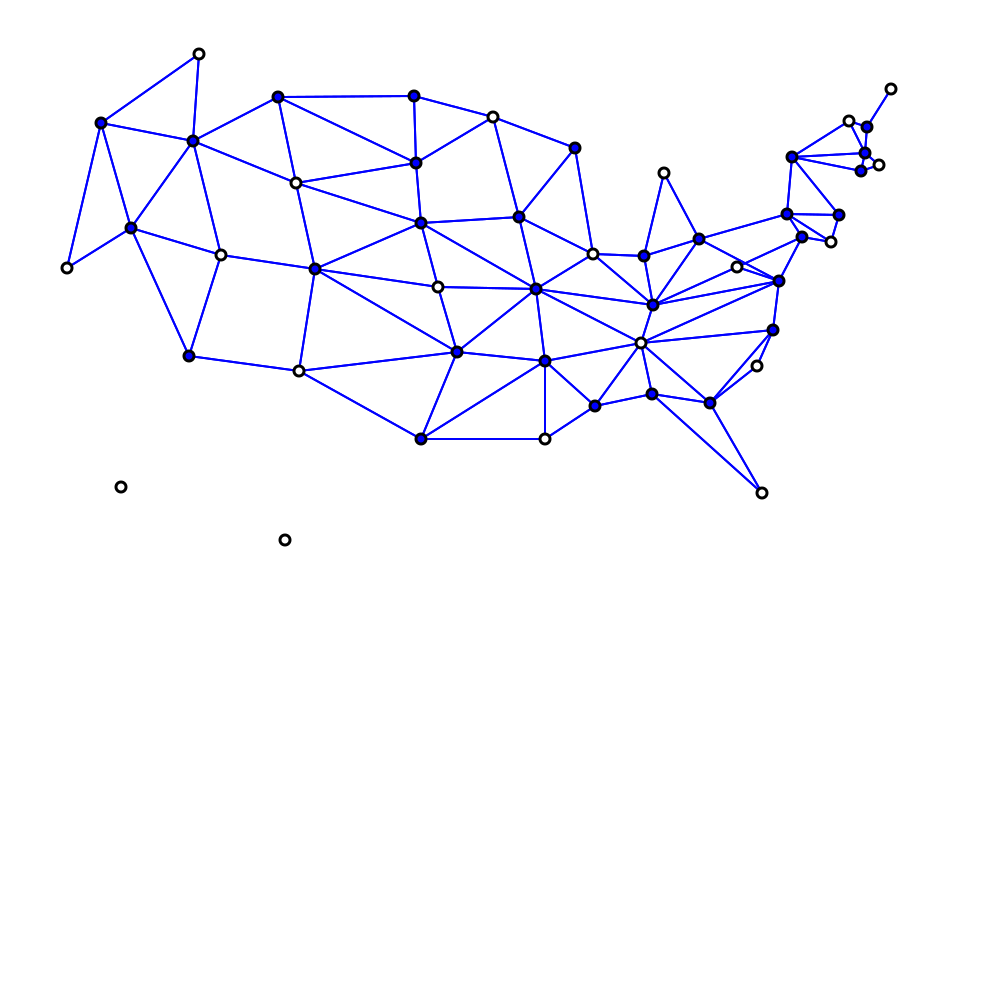
\includegraphics[scale=0.35]{usa}
    \end{minipage}%
    \begin{minipage}{.5\textwidth}
      \centering
      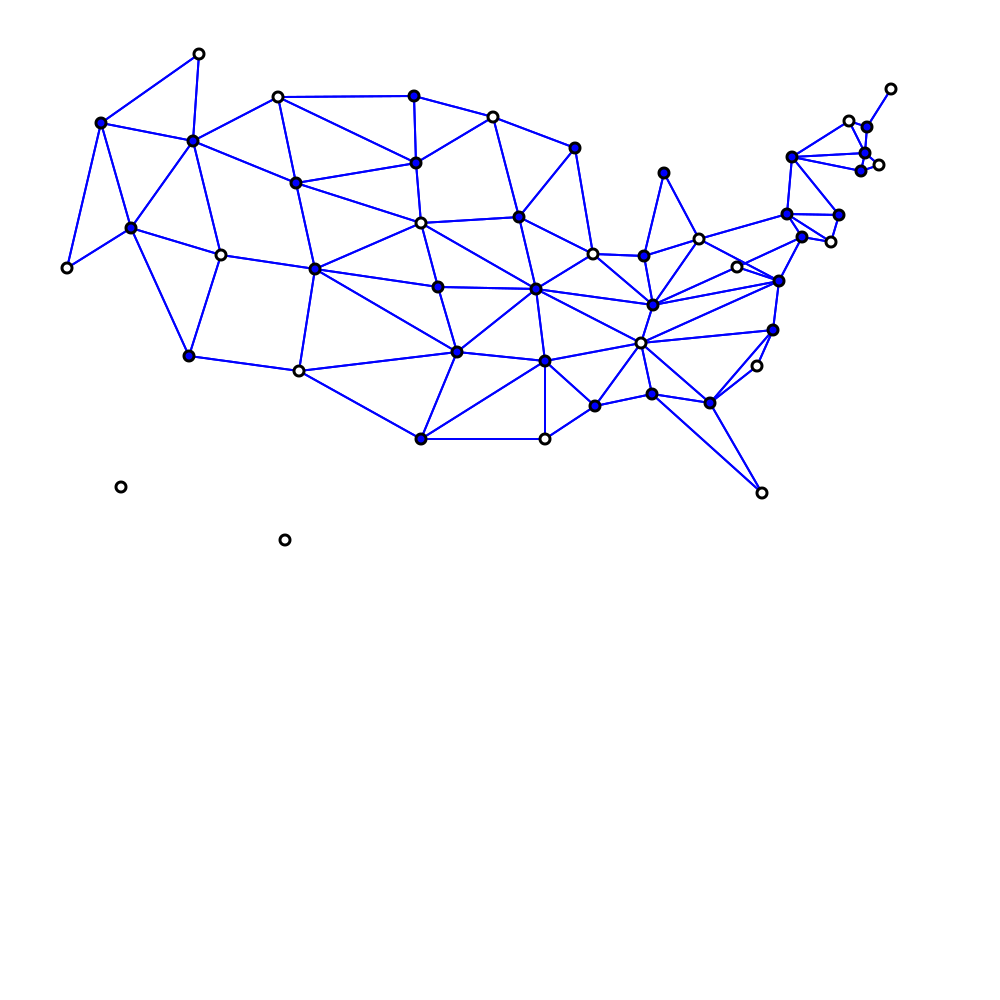
\includegraphics[scale=0.35]{usa2}
    \end{minipage}
    \caption{Dos cubiertas distintas del mapa de estados unidos pero con el mismo 
      costo\\
      ($T=50$, $\phi=0.8$, $L=20$, $\varepsilon = 0.001$, $\beta=1$, semillas 8 y 10)}
  \end{figure}

  \section{Discusión} \label{discussion}

  \section{Conclusión} \label{conclussion}
  
\end{document}
